% acl 分析时候突出回答2个事情1 为什么这个可以预测 可以做这事情本质原因是什么 2 有什么用 可以带来什么收益 有哪些应用价值  未来可以如何改进

\section{Analysis \& Insights}
\label{sec:analysis}

\begin{figure*}[!ht]
    \centering
    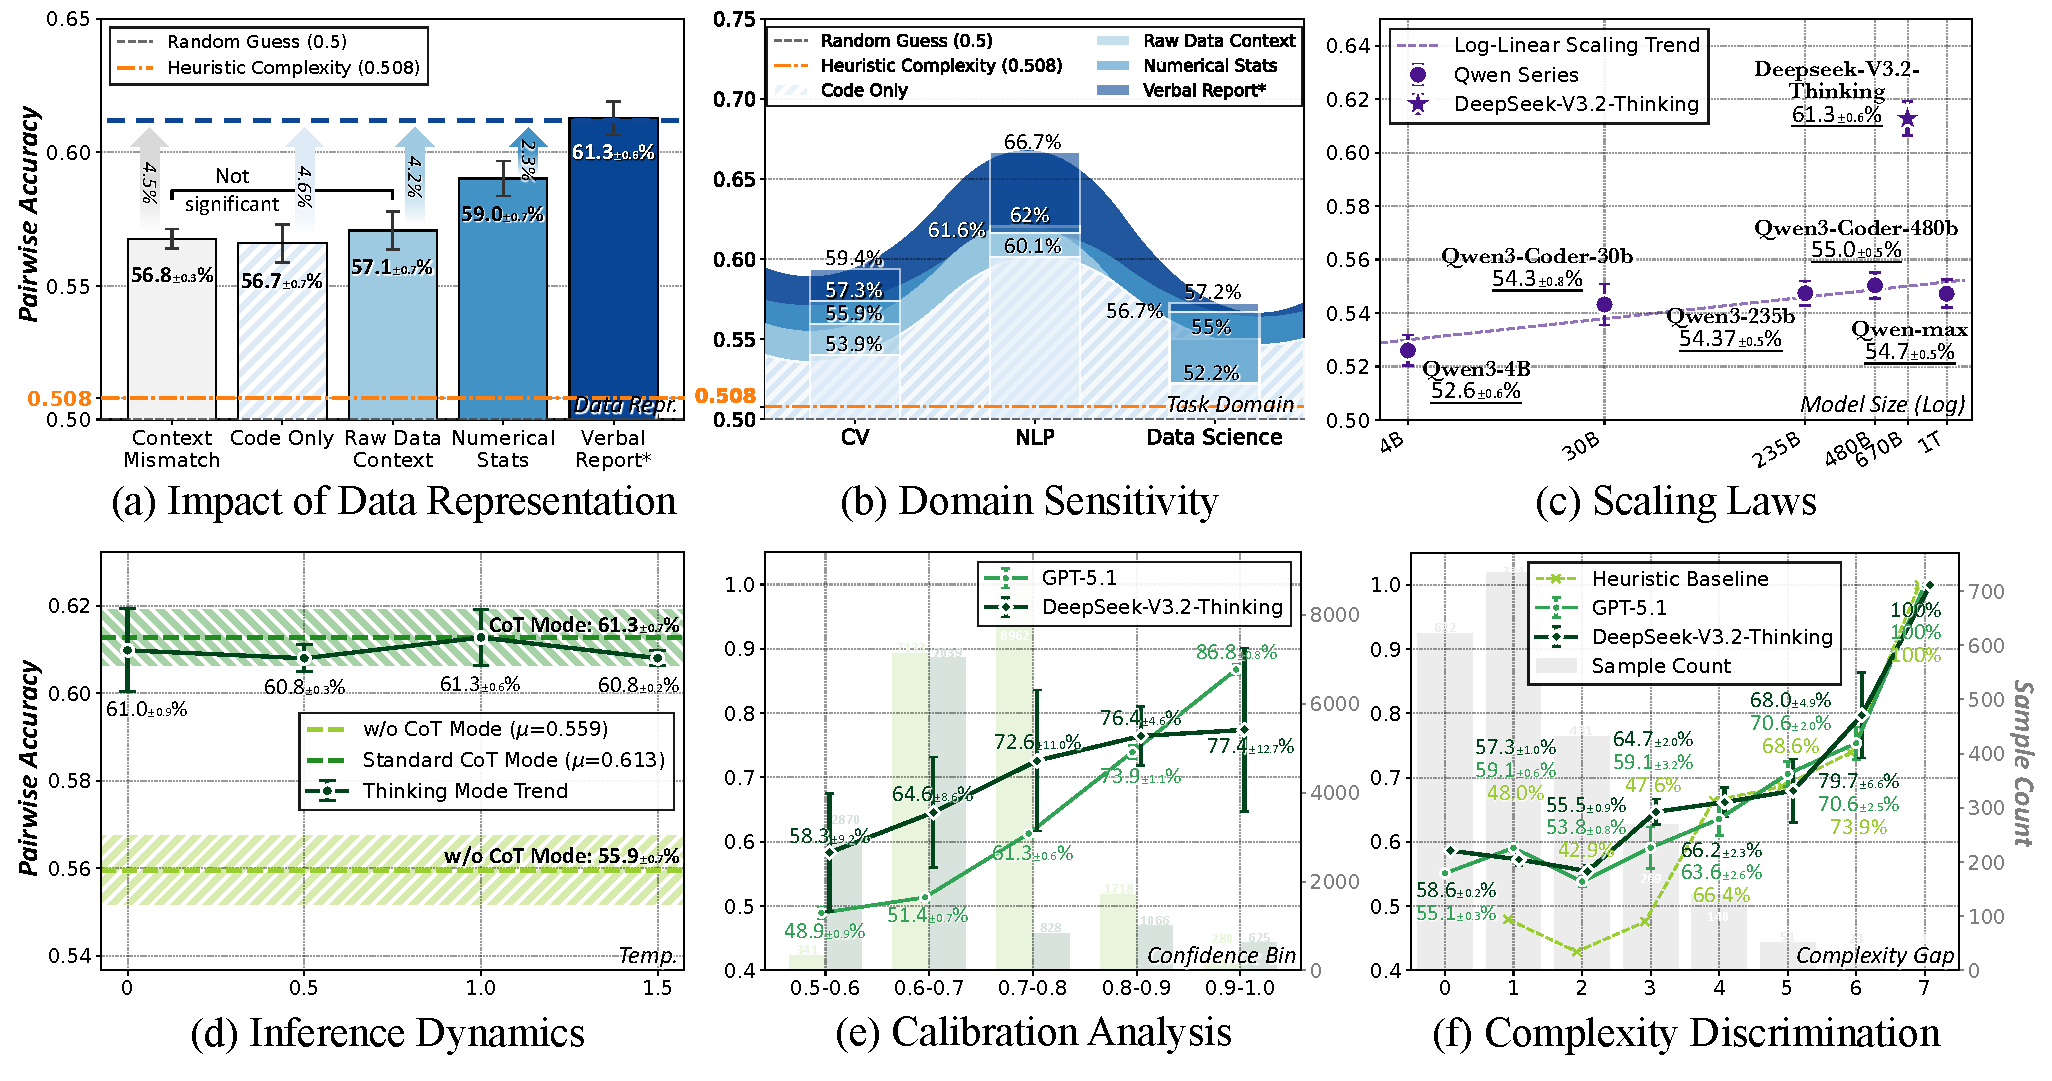
\includegraphics[width=1\linewidth]{figures/analysis_main.pdf}
    \caption{\textbf{Comprehensive Analysis of World Model Mechanisms and Capabilities.}
\textbf{(a) Impact of Data Representation:} Predictive success stems from semantic data understanding rather than complexity heuristics.
\textbf{(b) Domain Sensitivity:} The superiority of verbal reports remains consistent across domains.
\textbf{(c) Scaling Laws:} Accuracy decouples from pure parameter scaling.
\textbf{(d) Inference Dynamics:} Active reasoning outperforms direct answering with robust stability across temperatures.
\textbf{(e) Calibration Analysis:} Self-reported confidence correlates with accuracy.
\textbf{(f) Complexity Discrimination:} Accuracy scales with the complexity gap.}
    \label{fig:analysis}
\end{figure*}

\begin{insightbox}
    \textbf{{\usym{2660}} Discussion~\ref{subsec:rq1_representation}. The Gap Between Semantic and Numeric Spaces.}
    We observe that raw data yields insignificant gains over code-only input.
    We attribute this to the fact that continuous numerical values are \textbf{Weak-Semantic Symbols} that lack generalizable topological structure in the embedding space~\cite{davies2025languagemodelsembednumbers}.
    While language serves as a \textbf{Strong-Structural Symbol} carrying the compressed, empirical representations of human reasoning~\cite{Rytting2021leveragingtheinductivebias}, raw numbers appear to the model as unstructured high-entropy noise.
    Our verbalization strategy bridges this gap by projecting numeric data into the semantic manifold, injecting necessary inductive bias.
    Looking ahead, a fundamental resolution requires integrating \textbf{Symbolic Regression}~\cite{grayeli2024symbolicregressionlearnedconcept} to distill intricate logic directly from data.
\end{insightbox}


In this section, we deconstruct the mechanisms of the ``Implicit World Model'' through four pivotal research questions to answer: \textit{why can reasoning substitute for execution, and to what extent?}

While our representational analysis utilizes the full dataset, subsequent analysis (RQ2--RQ3) employs a focused subset capped at 15 solutions per task (2,292 pairs).
For ranking evaluations, we sample 105 instances per task to align with the pairwise baseline complexity ($C(15,2)$).

% ========================================================================
% RQ1: Data Representation
% ========================================================================
\subsection{RQ1: The Cognitive Mechanism of Data Representation}
\label{subsec:rq1_representation}

To distinguish genuine causal reasoning from syntactic memorization, we conducted a systematic study on input modalities (Figure~\ref{fig:analysis}(a)).
We instantiated four progressively enriched levels: \textit{Code Only} (task description + code), \textit{Raw Data} (appending initial samples), \textit{Numerical Stats} (execution logs from data analysis scripts), and \textit{Verbal Report} (full semantic analysis), alongside a \textit{Context Mismatch} control (pairing code with irrelevant context).

\paragraph{Finding 1: Predictive Success Stems from Semantic Data Understanding, Not Simple Complexity Heuristics.}
Our results refute a potential concern that LLMs merely rely on a complexity heuristic.
Figure~\ref{fig:analysis}(a) demonstrates a clear performance progression from the Heuristic Baseline (50.8\%) and Code Only (56.7\%) to Numerical Stats (59.0\%), peaking with Verbal Reports (61.3\%).
The insignificant gain of the Context Mismatch (56.8\%) over Code Only confirms that predictive success hinges on strict \textit{Semantic Alignment}.
The superiority of verbal narratives over raw statistics reveals that models operate primarily as \textit{rhetorical reasoners}, triggering an inference jump that is consistent across domains (Figure~\ref{fig:analysis}(b)).

% 核心逻辑：证明数据有效，Verbal Report最佳。
% 1. 展示 Baseline (Random/Heuristic) -> 证明任务很难，复杂度基于复杂度的启发式方法不行。
% 2. 展示 Code-only vs. Raw Data（仅提供任务描述和五条数据） -> 差异微乎其微，且未超过标准差 (56.6% vs 57.1%) -> 证明提供raw data没用，LLM 无法处理微观数据，Raw Data 在 CoT 模式下沦为噪声。
% 3. 展示Num-DA vs. Verbal report -> 展示llm对于文字的数据分析理解高于数字
% 4. 展示 Verbal Report 的跃升 (61.3%) -> 证明宏观语义是必须的。

% 为什么rawdata不行，a quantum-physics view

% 我们提出一种理论视角：当前的 LLM 在面对 ML 任务时，呈现出一种独特的**“认知二象性” (Cognitive Duality)**。

% 一方面是直觉模式（System 1），即模型试图通过内化的参数分布，对原始数据进行隐式的回归拟合——这是理想状态下 World Model 的终极形态。另一方面是逻辑模式（System 2），即通过思维链（CoT）对代码逻辑进行显式的因果推演。

% 然而，这种二象性并非平衡的。现代 LLM 的训练范式（尤其是 SFT 与 RLHF/RLAIF）已经发生了根本性偏移：模型被大量 CoT 数据微调，旨在优化推理轨迹的生成，而非像传统神经网络那样最小化回归损失（Regression Loss）。 这种训练归纳偏差（Inductive Bias）导致当且仅当“观测”（即要求生成推理）发生时，模型会瞬间从叠加态坍缩至其最擅长的逻辑推理模式。

% 这种坍缩带来的副作用是严重的：模型过度依赖被强化训练的逻辑推演能力，而其处理数值回归的直觉能力被抑制，导致原始数据的输入被忽略。这造成了方法论上的困境：微观数据的直接堆叠受限于上下文窗口，且与模型“重逻辑、轻回归”的训练本能不兼容。

% 因此，为了适配当前 LLM 以“逻辑推理”为主导的范式，我们将输入形式从 Raw Data 升级为 Verbal Report（数据报告）。这一转变本质上是将数据的微观特征预处理为宏观语义，从而将“数据理解”任务转化为模型擅长的“文本推理”任务，使 World Model 能够在保持 CoT 优势的同时，依然能够捕获数据的核心特性。

\begin{insightbox}
    \textbf{{\textcolor{red}{\usym{2665}}} Discussion~\ref{subsec:rq3_scaling}: The Illusion of Scaling on World-Blind Models.}
    We attribute scaling failures to \textbf{Information Scarcity}: static training corpora consist of code paired with merely \textit{trivial inputs} or abstract descriptions, lacking the \textit{large-scale data distributions} required for true dynamic execution interplay~\cite{liu2022mindseyegroundedlanguage}.
    While our results confirm that models can exploit sparse dynamic traces hidden in existing data, they remain fundamentally \textbf{World-Blind Learners}~\cite{floridi2025categoricalanalysislargelanguage}.
    To transcend this mere ``syntactic mimicry'', future scaling must pivot from static ingestion to \textbf{Interactive Simulation}, grounding agents in genuine causal feedback loops~\cite{benderkoller2020climbingtowardsnlu}.
\end{insightbox}

 

\subsection{RQ2: Capabilities, Boundaries, and Algorithmic Bias}
\label{subsec:rq2_boundary}

In this section, we  analyze the necessity of reasoning, domain sensitivity, generalization to ranking, and the reliability of its confidence.

\paragraph{Finding 2: Reasoning Unlocks Capabilities, Yet Distinct Cognitive Boundaries Persist Across Domains.}

Figure~\ref{fig:analysis}(d) identifies \textit{reasoning} as the primary engine, with the Thinking Mode (CoT)~\cite{deepseekai2025deepseekr1incentivizingreasoningcapability, openai2024openaio1card} ($61.3\%$) outperforming Direct Answering ($55.9\%$).
This performance remains robust across temperatures ($T \in [0, 1.5]$) and trajectory variance (see Appendix \ref{app:trajectory_variance}), implying an invariant logical core that relies on genuine reasoning rather than exploiting easy artifacts from the same agent run.
However, this capability is constrained by the problem landscape; Table~\ref{tab:final_compact_matrix_clean} reveals sharp performance stratifications across the Task-Solution matrix.
On the \textit{Task Dimension}, models demonstrate a preference for NLP ($66.9\%$) and Easy ($63.9\%$) paradigms.
Simultaneously, analysis on the \textit{Solution Dimension} reveals a comparison preference for Traditional ML within the \textit{Algo Era} ($64.5\%$), a ``Complexity Tax'' ($59.6\%$ on complex code), and a \textit{Granularity} bottleneck, where the model is more effective at distinguishing broad \textit{Cross-Algo} contrasts (comparing solutions with different algorithms, $62.8\%$).
Thus, while reasoning is indispensable, it faces limits when navigating intricate code logic or subtle intra class nuances.

Extending the scope to global \textbf{Listwise Ranking} further magnifies this limitation, as Table~\ref{tab:ranking_single_col} reveals a scalability defect where Accuracy@1 drops from the pairwise baseline ($61.3\% \to 31.1\%$) while Spearman Correlation hovers at a notably low level ($\rho \approx 0.23$), indicating that the model \textit{lacks global discrimination capability}, failing to sustain consistency beyond binary interactions.


\paragraph{Finding 3: The ``Implicit World Model'' Leverages Causal Reasoning Beyond Complexity Heuristics and Exhibits Robust Confidence Calibration.}

Tracing the \textit{Complexity Gap} in Figure~\ref{fig:analysis}(f) shows accuracy scales with distinction; crucially, the model's superiority over heuristics in low-gap scenarios proves it detects valid semantic signals rather than simple metrics.
Furthermore, Figure~\ref{fig:analysis}(e) demonstrates \textbf{Calibration}, where confidence correlates strictly with accuracy.
This reliability underpins the Section~\ref{sec:agent} gating mechanism, ensuring agents act with certainty.
\begin{table}
    \centering
    % 定义辅助命令：显示均值±标准差，并适当缩小字号
    \newcommand{\res}[2]{$#1_{\pm #2}$}
    
    % 调整表格样式
    \footnotesize  % 使用小字号
    \setlength{\tabcolsep}{3pt} % 极度压缩列间距 (默认是6pt)
    \renewcommand{\arraystretch}{1.25} % 增加行高，避免拥挤
    
    % 强制让表格适应单栏宽度 (linewidth)
    \resizebox{\linewidth}{!}{
        \begin{tabular}{c | c | c c c c}
            \toprule
            \textbf{Size} & \textbf{Corr.} & \multicolumn{4}{c}{\textbf{Accuracy@$k$ (\%)}} \\
            \cmidrule(l){3-6}
            \textbf{($N$)} & \textbf{Spr. $\rho$} & \textbf{$k$=1} & \textbf{$k$=2} & \textbf{$k$=3} & \textbf{$k$=4} \\
            \midrule
            
            % N=2
            \textbf{2} & \res{0.24}{0.01} & \res{61.3}{0.6} & -- & -- & -- \\
            
            % N=3
            \textbf{3} & \res{0.22}{0.00} & \res{43.4}{0.4} & \res{25.5}{0.4} & -- & -- \\
            
            % N=4
            \textbf{4} & \res{0.25}{0.00} & \res{35.0}{1.0} & \res{16.4}{0.7} & \res{10.2}{0.2} & -- \\
            
            % N=5
            \textbf{5} & \res{0.22}{0.00} & \res{31.1}{0.9} & \res{11.2}{0.3} & \res{4.9}{0.1} & \res{3.0}{0.2} \\
            
            \bottomrule
        \end{tabular}
    }
    
    \caption{\textbf{Ranking Performance.} 
    Listwise ranking metrics across varying list sizes $N$. 
    \textbf{Spr.}: Spearman Correlation ($\rho$). 
    \textbf{A@$k$}: Accuracy of the top-$k$ ranking positions (\%).
    ``--'' denotes undefined metrics where $k \ge N$.}
    
    \label{tab:ranking_single_col}
    
\end{table}

\begin{insightbox}
    \textbf{{\textcolor{orange}{\usym{2666}}} Discussion~\ref{sec:agent_motivation}. The Indirect Ceiling of Static Prediction.}
    We interpret 72.2\% as an \textbf{Indirect Epistemic Bound}, constrained by the \textit{Validation-Test Gap} and \textit{Limited Innovative Creativity}.
    Theoretically, since static prediction cannot outperform dynamic verification~\cite{rice1953classesofrecursively}, any gains beyond this saturation point represent the overfitting of distributional noise~\cite{dwork2015reusable}.
    Moreover, this ceiling exposes a deficit in \textit{Generative Innovation}: current LLMs hit a \textbf{Homogeneity Barrier}, producing \textit{functionally isomorphic} solutions that lack context-specific specialization~\cite{anil2024generativeaienhances}.
    Thus, lifting this bound relies on evolving base models to achieve the \textit{Genuine Innovation}.
\end{insightbox}

% ========================================================================
% RQ3: Scaling Law
% ========================================================================
\subsection{RQ3: Scaling Laws of Data-centric Solution Preference}
\label{subsec:rq3_scaling}

We evaluate the Qwen series across a spectrum from 4B to 1T to determine if predictive capability acts as an emergent scaling property.
Figure~\ref{fig:analysis}(c) details performance on five distinct checkpoints: 4B (\textit{Qwen3-4B-Instruct-2507}), 30B (\textit{Qwen3-Coder-30B-a3b-Instruct}), 235B (\textit{Qwen3-235B-a22b-Instruct-2507}), 480B (\textit{Qwen3-Coder-480B-a35b-Instruct}), and 1T (\textit{Qwen-Max}).

\paragraph{Finding 4: Predictive Accuracy Violates Standard Parameter Scaling Laws.}

Contrary to standard Parameter Scaling Laws, our results (Figure~\ref{fig:analysis}(c)) reveal a \textit{rapid saturation phenomenon}.
Within the Qwen series, performance sees diminishing returns after the initial 30B threshold, creating a statistical plateau that persists even at the 1T scale.
This trajectory implies a distinct ``capacity ceiling,'' suggesting that raw parameter scaling alone is insufficient for further gains in the \textit{Data-centric Solution Preference} task.
In contrast, the distinct superiority of DeepSeek-V3.2 ($61.3\%$) and GPT-5.1 ($58.8\%$) demonstrates that predictive power drives less from raw scale than from \textbf{reasoning-centric architectural paradigms}, implying that future gains will rely on specialized inference incentives rather than simple parameter expansion.

% 核心逻辑：模型越大，预测越准吗？
% 1. 模型系列：Qwen 家族 (4B -> >1T)。
% 2. 趋势分析：展示准确率随参数量的关系关系。
% 3. 结论：World Model 的预测能力不符合 Scaling Law。


\subsection{RQ4: Comparison with Human Judgment and Validation-Test Gap}
\label{subsec:rq4_cases}


To validate the model's reasoning depth, we conducted a qualitative analysis on the \textit{Google Quest Challenge} from main experiment, which is a multi-label subjective question-answering task.

\paragraph{Finding 5: The Model Outperforms Human Intuition by Rejecting Complexity Bias.}

In the case study of Figure~\ref{fig:case_study_quest}, the model surpassed human judgment by correctly prioritizing a simple LightGBM, whereas humans succumbed to the ``bigger is better'' bias by favoring a complex Deep Neural Network.
It successfully detects small-sample overfitting risks that humans missed, proving that data-grounded reasoning can effectively override superficial human biases.


\paragraph{The Validation-Test Gap.}
We further examine the reliability of execution-based validation metrics ($M_{val}$), derived from internal data splits, as proxies for test performance ($M_{test}$).
As shown in Table~\ref{tab:gap_analysis}, relying solely on $M_{val}$ yields an accuracy of only \textbf{72.2\%}.
This ceiling reveals a substantial \textbf{Validation-Test Gap} stemming from distributional shifts and validation overfitting.
Crucially, implicit reasoning partially mitigates this gap, offering a semantic safeguard that balances efficiency against the risk of metric-driven overfitting.

\begin{table}[h]
    \centering
    \small
    \begin{tabular}{lcc}
    \toprule
    \textbf{Signal Source} & \textbf{Cost} & \textbf{Acc. (\%)} \\
    \midrule
    Random Guess & - & 50.0 \\
    Exec. ($M_{val}$) & $\sim$Hours & 72.2 \\
    \textbf{LLM} & $\sim$Seconds & 61.5 \\
    \bottomrule
    \end{tabular}
    \caption{\textbf{Validation-Test Gap.} Local metrics ($M_{val}$) are noisy proxies for test performance ($M_{test}$), achieving only 72.2\% accuracy due to distribution shifts.}
    \vspace{-15pt}
    \label{tab:gap_analysis}
\end{table}